\documentclass[tikz,border=4pt]{standalone}
\usepackage{amsmath,amssymb}
\usetikzlibrary{arrows.meta}

\begin{document}
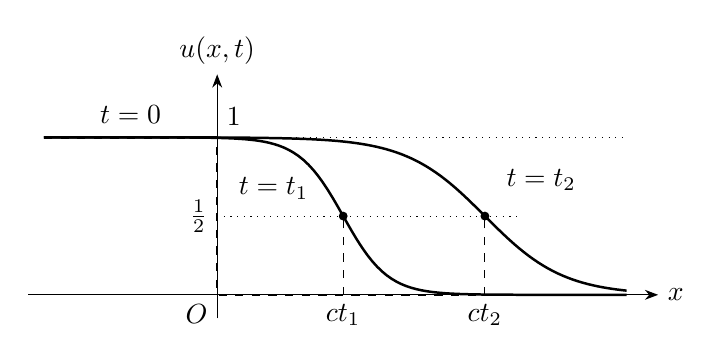
\begin{tikzpicture}[
  >=Stealth,
  font=\normalsize,
  axis/.style={line width=0.4pt},
  curve/.style={line width=0.9pt}
]
  % Axes
  \draw[axis,->] (-2.4,0) -- (5.6,0) node[right] {$x$};
  \draw[axis,->] (0,-0.3) -- (0,2.8) node[above] {$u(x,t)$};
  \node[below left] at (0,0) {$O$};
  \node[above right] at (0,2.02) {$1$};
  \node[left] at (0,1.0) {$\tfrac{1}{2}$};
  \draw[axis,dotted] (-2.2,2.0) -- (5.2,2.0);
  \draw[axis,dotted] (0,1.0) -- (3.8,1.0);

  % t = 0 step function (dashed)
  \draw[curve,dashed] (-2.2,2.0) -- (0,2.0) -- (0,0) -- (5.2,0);
  \node[above] at (-1.1,2.05) {$t = 0$};

  % t = t_1 > 0: centered at x = 1.6, width ~ 0.65
  \draw[curve,domain=-2.2:5.2,samples=120]
    plot (\x, {2.0/(1 + exp(min(8, max(-8, 2.3*(\x - 1.6)/0.65))))});
  \fill (1.6,1.0) circle (1.6pt);
  \draw[axis,dashed] (1.6,0) -- (1.6,1.0);
  \node[below] at (1.6,0) {$ct_1$};
  \node[left] at (1.28,1.35) {$t = t_1$};

  % t = t_2 > t_1: centered at x = 3.4, width ~ 1.15
  \draw[curve,domain=-2.2:5.2,samples=120]
    plot (\x, {2.0/(1 + exp(min(8, max(-8, 2.3*(\x - 3.4)/1.15))))});
  \fill (3.4,1.0) circle (1.6pt);
  \draw[axis,dashed] (3.4,0) -- (3.4,1.0);
  \node[below] at (3.4,0) {$ct_2$};
  \node[above right] at (3.55,1.2) {$t = t_2$};
\end{tikzpicture}
\end{document}
